\documentclass[12pt, a4papre]{article}
\usepackage[catalan]{babel}
\usepackage[unicode]{hyperref}
\usepackage{amsmath}
\usepackage{amssymb}
\usepackage{amsthm}
\usepackage{xifthen}
\usepackage{siunitx}
\usepackage{xcolor}
\usepackage{float}
\usepackage{listings}
\usepackage{setspace}
\usepackage{graphicx}
\usepackage{tikz,lipsum,lmodern}
\usepackage[most]{tcolorbox}
\usepackage{circuitikz}
\usepackage{indentfirst}
\usepackage{verbatimbox}
\definecolor{mygreen}{RGB}{28,172,0} % color values Red, Green, Blue
\definecolor{mylilas}{RGB}{170,55,241}

\graphicspath{ {./images/} }


\newcommand{\norm}[1]{\lvert #1 \rvert}

\hypersetup{
    colorlinks = true,
    linkcolor = blue
}

\author{Daniel Vilardell\\
	   Igor Yuziv}
\title{Memoria practica 1 DGD}
\date{17-10-2020}

\begin{document}
	\maketitle
	Aquesta primera practica es divideix en dos parts, la part a i la part b. La primera part es basa en aprendre com funciona el programa Quartus II a partir de fer un multiplexor  2:1 per a bussos de 4 bits i verificar el seu funcionament sobre la placa DE2. En la segona part, aplicant el coneixement adquirit en la primera, construim una calculadora que permet multiplicar dos nombres de 4 bits en CA2.
	
	En aquesta memoria explicarem detalladament la construccio de cada component i com s'usa per a assolir els objectius proposats.

	\newpage
	\section{Primera part}
	
	\newpage
	\section{Segona part}
	\textbf{\large{Convertidor de CA2 de 4 a 8 bits}}
	
	Aquest component es ben simple i s'usara per a poder fer el producte de dos nombres en CA2 ja que el resultat de la multiplicació és sempre un nombre de 8 bits. El que fa es agafar el bit de mes pes de la entrada i el repeteix als bits de mes pes seguents. La rao per la que funciona aquesta idea ja està vista al previ
	
	\begin{figure}[H]
		\begin{center}
		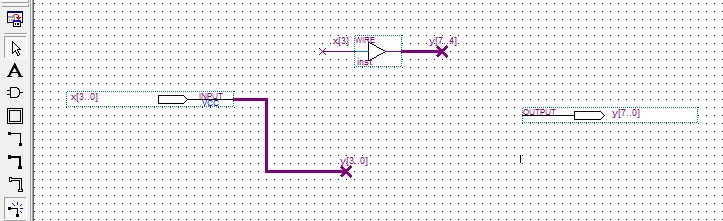
\includegraphics[width=150mm]{CA2_4_a_8.jpeg}
		\end{center}
	\end{figure}
	
	
	\textbf{\large{Multiplicador 8x1}}
	
	Aquest component muliplica un nombre de 8 bits per  un nombre de 1 bit. Per tant la sortida sera el nombre de 8 bits entrat si l'altre nombre es 1, i 0 altrament.
	\begin{center}
	FOTO DEL COMPONENT
	
	FOTO DE LA SIMULACIO
	\end{center}
	
	\textbf{\large{Multiplicador i sumador}}
	
	Aquest component te la funcio de multiplicar un nombre de 8 bits per un de 1 usant el component mencionat anteriorment per després sumar el resultat amb un altre nombre de 8 bits que ve a l'entrada. Això es fara servir per a fer la multiplicacio classica que es basa en multiplicar un per un els bits del nombre de baix i sumar amb els anteriors sempre treient el bit de menys pes. Es per aixo que les sortides del component son per una banda el bit de menys pes que s'usara per a posar al resultat, i per altra els 7 bits de mes pes resultants de la suma. 
	
	\begin{center}
	FOTO DEL COMPONENT
	\end{center}
	
	\textbf{\large{Multiplicador binari de 8 bits}}
	
	Aquest component multiplica dos nombres de 8 bits a partir de posar en serie els muliplicadors i sumadors comentats abans. La entrada son dos nombres de 8 bits, i a cada entrada dels 8 components en serie s'hi posarà el nombre de dalt, es a dir A[7..0], el bit que toqui del nombre de baix, B[i] i finalment se li entrarà la suma de les anteriors multiplicacions extreient el bit de menys pes. Aquest bit de menys pes anirà al nombre de 16 bits que hi ha a la sortida. Finalment quan s'arriba al últim component s'introdueix tota la sortida (la suma i el bit de menys pes) a la sortida general del component.
	
	\begin{center}
	FOTO DEL COMPONENT
	
	FOTO DE LA SIMULACIO
	\end{center}
	
	\textbf{\large{Multiplicador CA2 de 4 bits}}
	
	Aquest component multiplica dos nombres en CA2 de 4 bits. Per a fer això primer els transforma a CA2 de 8 bits amb el primer component mencionat, per a despres introduirlo al multiplicador binari de 8 bits. Tot i que la sortida es de 16 bits, nomes ens interessen els 8 bits de menys pes ja que al multiplicar dos nombres de 4 bits, el resultat maxim tindrà 8 bits.
	
	\begin{center}
	FOTO DEL COMPONENT
	
	FOTO DE LA SIMULACIO
	\end{center}
	
	\textbf{\large{Adaptador de signe}}
	
	Aquest component te la finalitat de veure si el valor es negatiu o positiu i en el cas de que sigui negatiu, encen el segment de la placa corresponent per a que pugui ser visualitzat.
	
	\begin{center}
	FOTO DEL COMPONENT
	\end{center}
	
	\textbf{\large{Convertidor CA2 de 4 bits al seu modul}}
	
	Aquest component es el que ens permetrà extreure el modul de un nombre en CA2 de 4 bits per tal de representarlo a la placa.
	
	\begin{center}
	FOTO DEL COMPONENT
	\end{center}
	
	\textbf{\large{Multiplicador final per a visualització}}
	
	Aquesta multiplicació final te tres branques, una per a la visualització del primer nombre entrat, una per a la visualització del segon i finalment una per a visualitzar el resultat. La entrada sera de dos nombres de 4 bits als que assignarem pins de la placa. 
	
	La primera branca i la segona funcionen igual així que només explicarem una d'elles. 
	\begin{enumerate}
	\item Quan s'entra un nombre en CA2 de quatre bits, primer determinem el signe amb el adaptador de signe. Aquesta sortida ja va directe a la placa i mostra el signe.
	\item Després de determinar el signe es converteix el nombre en CA2 al seu modul.
	\item Quan ja tenim el modul l'introduim a un component facilitat per la assignatura que converteix nombres binaris de 4 bits a BCD de 7 segments. Aquesta sortida també va directe a la placa i mostra el nombre.
	\end{enumerate}
	
	La tercera i ultima branca funciona de la següent manera:
	\begin{enumerate}
	\item Primer s'introdueixen els dos nombres al multiplicador CA2 de 4 bits, el qual dona el seu producte en CA2.
	\item S'extreu el signe a partir del bit de mes pes i es mostra a la placa usant el adaptador de signe.
	\item La sortida del producte s'introdueix dins del component facilitat també per la assignatura que et dona el BCD de un nombre de 8 bits.
	\item Els primers 4 bits seran el primer nombre de la sortida, així doncs aquest nombre es passa a BCD de 7 segments i es mostra a la placa.
	\item Finalment es fa el mateix pels 4 ultims bits, els de menys pes, i es mostra a la placa.
	\end{enumerate}
	
	\begin{center}
	FOTO DEL COMPONENT
	
	FOTO DE LA SIMULACIO
	\end{center}
	
	\newpage
	\section{Tercera part(extra)}
	
	Un cop implementada la calculadora que permet fer el producte de dos nombres en CA2, ara sens proposa que montem un component que a partir de tres entrades, A B i selop tregui la sortida seguent:
	
	\begin{itemize}
	\item $A\cdot B$ si selop $=00$
	\item $A^2$ si selop $=01$
	\item $B^2$ si selop $=10$
	\item$2^A\cdot2^B$ si selop $=11$
	\end{itemize}
	
	Cal tenir en compte en primer lloc que la sortida es de 8 bits, i per tant la sortida $2^A\cdot2^B$ no podra mostrar totes les sortides possibles. Tenint en compte que com la sortida es en CA2, nomes disposem de 7 bits i per tant nomes podrem representar totes aquelles sortides tals que $A+B \leqslant 7$. 
	
\end{document}